\section{Introduction}\label{sec:intro}
In this era an abundant resource became available, that is a large amount of
structured and unstructured data.
\textbf{Machine Learning} (\textbf{ML}) has evolved as a branch of artificial
intelligence, which envisages the development of self-learning algorithms,
capable of acquiring knowledge from data, with the aim of making predictions.
Instead of requiring a human presence, able to manually enact the rules and
build models for the analysis of large amounts of data, machine learning offers
a more efficient alternative to capture the knowledge inherent in the data,
with the aim of gradually improving the performance of forecasting models and
make data driven decisions.
In this section we will examine the three different types of machine learning:
\emph{supervised learning}, \emph{unsupervised learning} and
\emph{reinforcement learning}.
Where we will show the fundamental differences between these different types of
learning.\cite{raschka2016machine}
%
\subsection{Supervised learnig}\label{subsec:supervised-learnig}
The main purpose of supervised learning is to derive a model from 
training data, which allows us to make predictions for data that are not
available or future.
Here the term with supervision refers to the fact that the
set of samples the desired output signal labels are already known.
A supervised learning task, based on discrete class labels, is also called a
classification task.
Another supervised learning subcategory is regression, where the resulting
signal is a continuous value.
Classification is a sub-category of supervised learning, where the goal is to
provide class category labels for new instances, based on observations made in
the past.
These labels are discrete, unordered values ​​that can be considered as
belonging to a group of instances.
However, the set of class labels does not necessarily have to be a binary
nature.
The predictive model identified by a supervised learning algorithm can consider
each class label that is present in the learning dataset of a new instance that
is not labelled.
A typical example of \emph{multi-class classification} is the recognition of
hand-written text.\cite{raschka2016machine}
%
\begin{figure}[!h]
\centering
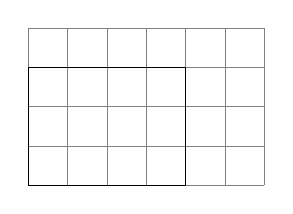
\begin{tikzpicture}
 \draw [help lines] (0,0) grid [step=0.5] (3,2);
 \draw (0,0) rectangle ++(2cm,1.5cm);
\end{tikzpicture} 
\caption{supervised learning scheme} 
\label{fig:supervised-learning-scheme}
\end{figure}
%
\subsection{Reinforcement learnig}\label{subsec:reinforcement-learnig}
Another type of machine learning and reinforcement learning.
Here the goal is to develop a system (\emph{agent}) for people who improve
their performance based on interactions with the environment.
Since, typically, information relating to the current state of the environment
including also a so-called \emph{reward} signal, we can consider strengthening
learning as an example of supervised learning.
However, in reinforcement learning, this feedback is not the correct label or
truth value, but the measure of the quality with which the action was measured
has no reward function.
Through interaction with the environment, an agent can then use reinforcement
learning to learn a series of actions that maximize this reward through a
trial-and-error exploratory approach or deliberative planning.\cite{raschka2016machine}
%
\begin{figure}[!h]
\centering
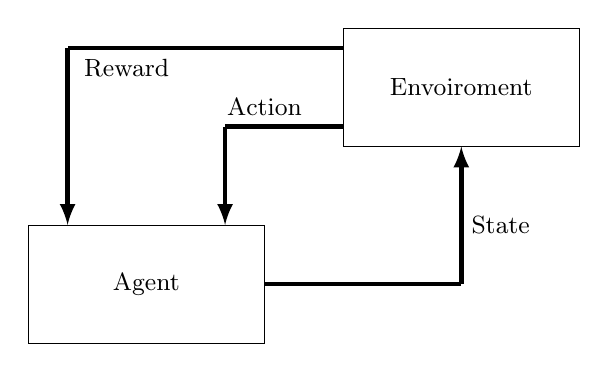
\begin{tikzpicture}[>=latex]
 %\draw [help lines] (0,0) grid [step=0.5] (8,4);
 \draw (0.5,0) rectangle ++(3cm, 1.5cm);
 \draw (4.5,2.5) rectangle ++(3cm,1.5cm);
 %\node [draw] (1.5,2) {Agent};
 \coordinate [label={[font=\small]center:Agent}] (A) at (2,0.75);
 \coordinate [label={[font=\small]center:Envoiroment}] (E) at (6,3.25);
 \draw [-, ultra thick] (3.5,0.75) -- (6,0.75);
 \draw [->, ultra thick] (6,.75) -- (6,2.5);
 \coordinate [label={[font=\small]center:State}] (S) at (6.5,1.5);
 %
 \draw [-, ultra thick] (4.5,2.75) -- (3,2.75);
 \draw [->, ultra thick] (3,2.75) -- (3,1.5);
 \coordinate [label={[font=\small]center:Action}] (T) at (3.5,3);
 %
 \draw [-, ultra thick] (4.5,3.75) -- (1,3.75);
 \draw [->, ultra thick] (1,3.75) -- (1,1.5);
 \coordinate [label={[font=\small]center:Reward}] (R) at (1.75,3.5);
\end{tikzpicture} 
\caption{reinforcement learning scheme} 
\label{fig:reinforcement-learning-scheme}
\end{figure}
%
\subsection{Unsupervised learning}\label{subsec:unsupervised-learning}
In supervised learning, we know in advance the correct answer when we describe
our model, while in reinforcement learning we define a measure, or reward, for
the specific actions performed by the agent.
In unsupervised learning, on the other hand, we are dealing with unlabelled data
or data from the unknown structure.
Using unsupervised learning techniques, we are able to observe the structure of
our data, to extract meaningful information from them without being able to
rely on the guide nor a variable known relative result, nor a reward function.
Clustering is an exploratory technique of data analysis that allows us to
organize a series of information within meaningful groups (\emph{cluster})
without having any previous knowledge of memberships in such groups.
Each cluster that can be derived during the analysis defines a group of objects
that share a certain degree of similarity, but which are more dissimilar than
the objects present in the other clusters, which is why clustering is sometimes
called \emph{``unsupervised classification"}.
Clustering is an excellent technique for structuring information to identify
meaningful relationships in the data.\cite{raschka2016machine}
%
\begin{figure}[!h]
\centering
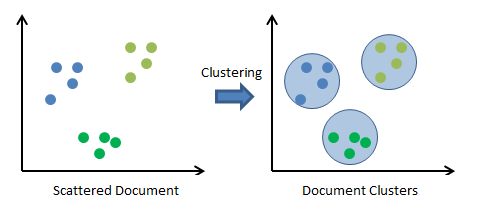
\includegraphics[width=\linewidth]{cluster}
\caption{example of clustering}
\label{fig:unsupervised-learning-scheme}
\end{figure}
%
\subsection{Prerequisites}
\label{subsec:rerequisites}
The code requires Python 3.5.2 or higher (version 3.7 is not supported) to be
installed on a MacOS, Linux or Windows system.
Referring to essential libraries dedicated to the scientific group, including
SciPy, NumPy, scikit-learn, matplolib and pandas.
We will add the TensorFlow-gpu library for efficient training of neuronal
networks on GPU units.
